\section{Installing PGP on Windows}

To complicate matters a little - PGP is the protocol used for encrypting
e-mail by various softwares. To get PGP to work with Thunderbird we need
to install GPG - a free software implementation of PGP \emph{and}
Enigmail - an extension of Thunderbird that allows you to use
GPG\ldots{} Confused?! Don't worry about it, all you have to know is how
to encrypt your email with PGP and you need to install \emph{both} GPG
and Enigmail. Here is how to do it\ldots{}

\subsection{Installing PGP (GPG) on Microsoft Windows}

The GNU Privacy Guard (GnuPG) is software which is required to send PGP
encrypted or signed emails. It is necessary to install this software
before being able to do any encryption.

Head to the website of the Gpg4win project. Go to
\href{http://gpg4win.org/}{http://gpg4win.org/}

On the left side of the website, you will find a `Download' link. Click
on it.

\begin{figure}[htbp]
\centering

\includegraphics{gpg_win.png}
\caption{GPG Windows}
\end{figure}

This will take you to a page where you can download the Gpg4Win. Click
on the button which offers you the latest stable version (not beta) of
Gpg4Win.

\begin{figure}[htbp]
\centering
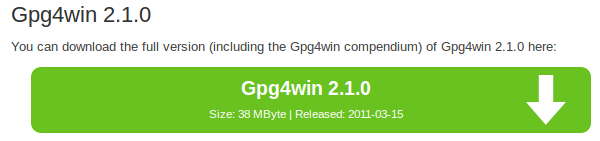
\includegraphics{gpg_win_2.png}
\caption{GPG Windows}
\end{figure}

This will download you an .exe file. Depending on your browser, you may
have to double-click on this downloaded file (which will be called
something like \verb!gpg4qin-2.1.0.exe!) before something happens.
Windows will ask you if you are sure you want to install this program.
Answer yes.

Then complete the installation by agreeing to the license, choosing
appropriate language and accepting the default options by clicking
`Next', unless you have a particular reason not to.

The installer will ask you where to put the application on your
computer. The default setting should be fine but make a note of it as we
may need this later. Click on `Next' when you agree.

\subsection{Installing with the Enigmail extension}

After you have successfully installed the \textbf{PGP} software as we
described above you are now ready to install the \textbf{Enigmail}
add-on.

Enigmail is a Thunderbird add-on that lets you protect the privacy of
your email conversations. Enigmail is simply an interface that lets you
use PGP encryption from within Thunderbird.

Enigmail is based on public-key cryptography. In this method, each
individual must generate her/his own personal key pair. The first key is
known as the private key. It is protected by a password or passphrase,
guarded and never shared with anyone.

The second key is known as the public key. This key can be shared with
any of your correspondents. Once you have a correspondent's public key
you can begin sending encrypted e-mails to this person. Only she will be
able to decrypt and read your emails, because she is the only person who
has access to the matching private key.

Similarly, if you send a copy of your own public key to your e-mail
contacts and keep the matching private key secret, only you will be able
to read encrypted messages from those contacts.

Enigmail also lets you attach digital signatures to your messages. The
recipient of your message who has a genuine copy of your public key will
be able to verify that the e-mail comes from you, and that its content
was not tampered with on the way. Similarly, if you have a
correspondent's public key, you can verify the digital signatures on her
messages.

\subsection{Installation steps}

To begin installing Enigmail, perform the following steps:

\begin{enumerate}[1.]
\item
  Open \textbf{Thunderbird}, then \verb!Select Tools > Add-ons! to
  activate the \emph{Add-ons} window; the Add-ons window will appear
  with the default \emph{Get Add-ons} pane enabled.
\item
  Enter enigmail in the search bar, like below, and click on the search
  icon.
\end{enumerate}
\begin{figure}[htbp]
\centering
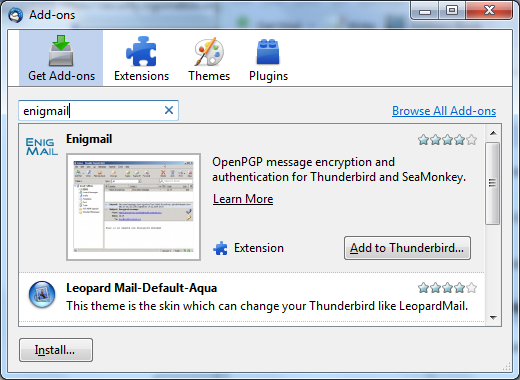
\includegraphics{enigmail_inst_1.png}
\caption{Enigmail Install}
\end{figure}

\begin{enumerate}[1.]
\setcounter{enumi}{2}
\item
  Simply click on the `Add to Thunderbird' button to start the
  installation.
\item
  Thunderbird will ask you if you are certain you want to install this
  add-on. We trust this application so we should click on the `Install
  now' button.
\end{enumerate}
\begin{figure}[htbp]
\centering
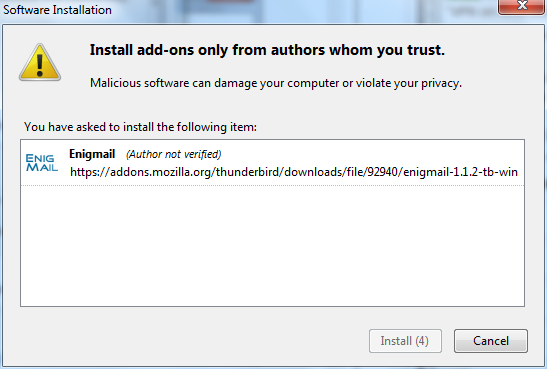
\includegraphics{enigmail_inst_2.png}
\caption{Enigmail Install}
\end{figure}

\begin{enumerate}[1.]
\setcounter{enumi}{4}
\item
  After some time the installation should be completed and the following
  window should appear. Please click on the `Restart Thunderbird'
  button.
\end{enumerate}
\begin{figure}[htbp]
\centering
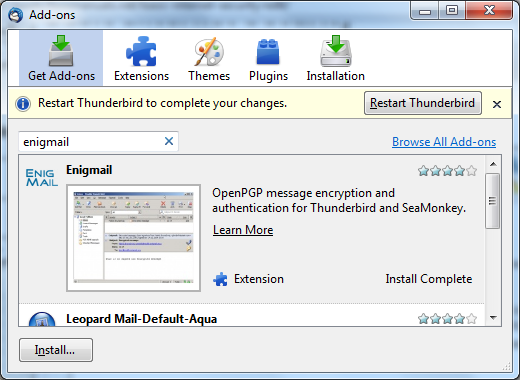
\includegraphics{enigmail_inst_3.png}
\caption{Enigmail Install}
\end{figure}

